\subsection{Decision Model 적용에 따른 근거 선택 성능 변화 (RQ1)}

\label{sec:ch4_2}

Jev 교체로 평균 최종 근거 F1은 3.19점(CI [+0.75, +5.68]점), Recall은 2.95점(CI [+0.39, +5.51]점) 높아졌으나, 필요한 근거를 모두 확보한 문항의 증가는 0과 구분되지 않았다(조건별 값은 S2). 근거 평가는 정답 근거(gold)와의 문자열 집합 일치를 보므로 정답 외 근거의 법률적 타당성은 판정하지 않는다.

\begin{figure}[H]
\centering
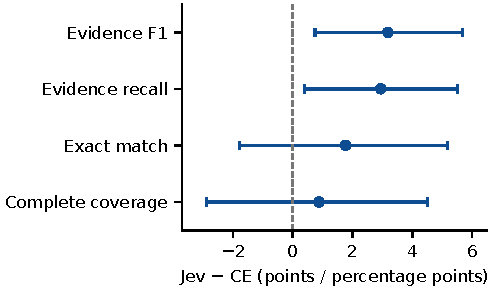
\includegraphics[width=\linewidth]{research/chapter4/figures/section-figures-v1/fig_4_2_evidence_effects_column.pdf}
\caption{최종 근거 성능의 Jev$-$CE 차이와 탐색적 95\% CI. Complete coverage는 완전 회수이며, EM·완전 회수율 차이는 \%p, 나머지는 점 단위이다.}
\label{fig:ch4_2}
\end{figure}

반면 EM(선택 집합과 gold의 완전 일치)은 27.88\%에서 29.65\%로, 완전 회수율(정답 외 근거가 있더라도 gold를 빠짐없이 포함)은 34.07\%에서 34.96\%로 증가하는 데 그쳤고, 두 차이의 CI는 0을 포함하였다(그림~\ref{fig:ch4_2}).

문항별 F1은 Jev 우세 32개, 동일 177개, CE 우세 17개였다. 데이터셋 hop 라벨별 F1은 1-hop 78.07$\to$76.90(Jev 우세/동일/CE 우세 0/56/1문항), 2-hop 53.33$\to$57.24(20/95/12), 3-hop 47.91$\to$54.83(12/26/4)으로, 전체 차이는 주로 2·3-hop 문항에서 관측되었다. 이는 집단별 관측 평균이며 효과 차이를 검정한 결과는 아니다. 고유 gold 386개 중 27개(29문항)는 corpus에서 동일 문자열을 찾을 수 없었으나 분석에서 제외하지 않았다(S6).

공개 코드 CE의 F1은 48.72점으로 수정 CE보다 9.85점 낮았다(해석 범위는 S2).
